\section{Introduction}
\label{sec:introduction}
\subsection{Background}
\paragraph{}Face recognition can be done using Artificial intelligence for applications such as control of access, which will be the main focus of this project. It proves to be better than the state of the art method of control access i.e. manual check of Identification cards at the gate. Although this technology is not yet 100 %, 
a thorough training of models can ultimately reach very high levels of accuracy.
\paragraph{}Another application of Face Recognition technology is in generating sign sheets for different lectures at the university. Therefore, Visage will seek to incorporate face recognition with attendance registration.
%\begin{figure}
%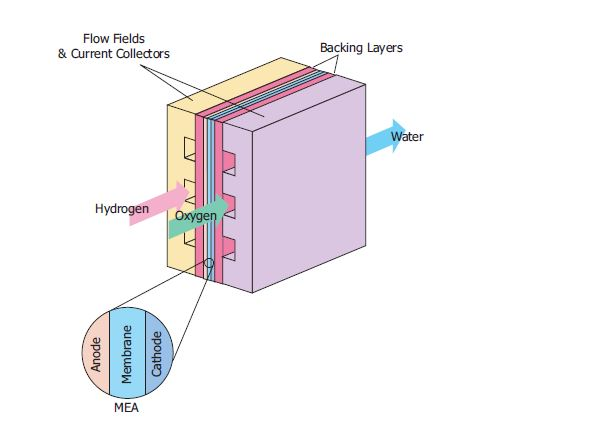
\includegraphics{Figures/Figure3}
%\caption{Fuel Cell Structure
%\cite{pukrushpan_modeling_2003}}
%\end{figure}

\subsection{Problem Statement}
\paragraph{}Monitoring students enterring an institution is an important security step both for the other students as well as for the school property. It is a way to keep off intruders and prevent potential attacks. This monitoring is currently done manually i.e. students have to show their IDs every time they want to enter the school. Another important practice in university education is the signing of sign sheets. This enables the lecturers to keep track of students who attend or don't attend classes. A minimum percentage of classes has to be attained for one to sit for exams.

\paragraph{}These two activities, access control and class attendance, are limited in various aspects. For access control, a student may lose their IDs which will have them refused access into the school despite their frequency there. Also, intruders may use student IDs to access the school. For class attendance, the inaccuracy is due to the prevalent exercise of students signing for their counterparts who do not attend classes. This leaves lecturers at a fix at the end of the semester when they cannot explain low grades among some of their students.

\paragraph{}To solve these two issues, Visage is going to be a face recognition device with attendance generation capabilities. The device will be portable and mountable on the wall.

\subsection{Objectives}
\subsubsection{Main Objective}
To develop a rugged Face recognition device for access control and attendance monitoring
\subsubsection{Specific Objectives}
\begin{enumerate}
\item To design and fabricate a rugged housing for the electronic components of Visage.
\item To build models for Face Recognition.
\item To train the models using data from a given population i.e. volunteers
\item To deploy and showcase Visage at the Tech Expo 12.0
\end{enumerate}

\subsection{Justification of Project}
\paragraph{}\begin{enumerate}
\item Circumstances, like Covid-19, may arise that may need registration of people entering social places e.g. churches. These registrations should not lead to very long queues as was the case previously.
\item Face recognition devices for access control exist but may be expensive. Visage will aim at beingg cost-effective while maintaining or surpassing the efficiency levels.
\item Visage is an opportunity for young African scholars like ourselves to not only learn but also to build using Artificial Intelligence.
\item If Visage is successful it will put JKUAT on the AI map.
\item Employment opportunities for the future for the many data and Machine Learning engineers.
\end{enumerate}
